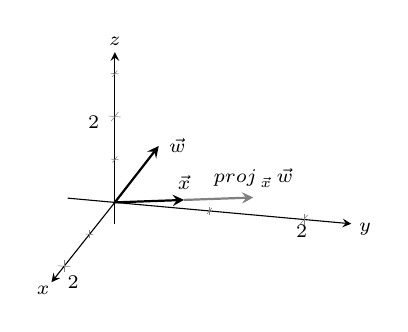
\begin{tikzpicture}
\begin{axis}%
[width=175pt,tick label style={font=\scriptsize},axis on top,
			axis lines=center,
			view={105}{30},
			name=myplot,
			%xtick=\empty,
			%ytick=\empty,
			%ztick=\empty,
			minor x tick num=1,
			minor y tick num=1,
			minor z tick num=1,
			ymin=-.5,ymax=2.5,
			xmin=-.5,xmax=2.5,
			zmin=-.5, zmax=3.5,
			every axis x label/.style={at={(axis cs:\pgfkeysvalueof{/pgfplots/xmax},0,0)},xshift=-3pt,yshift=-3pt},
				xlabel={\scriptsize $x$},
			every axis y label/.style={at={(axis cs:0,\pgfkeysvalueof{/pgfplots/ymax},0)},xshift=5pt,yshift=-2pt},
				ylabel={\scriptsize $y$},
				every axis z label/.style={at={(axis cs:0,0,\pgfkeysvalueof{/pgfplots/zmax})},xshift=0pt,yshift=4pt},
				zlabel={\scriptsize $z$},
>=stealth%
]


%\addplot3[domain=-.1:1,y domain=-.1:1,surf,faceted color=black!20,samples=10,black!10] {-.1*x+y+1};
\threedlines{2}{1}{3}
\threedlines{1}{1}{1}
\threedlines{2}{2}{2}

\draw[>=stealth,->,thick] (axis cs:0,0,0) -- (axis cs: 2,1,3) node [right] {\scriptsize $\vec w$};

\draw[>=stealth,->,thick] (axis cs:0,0,0) -- (axis cs: 1,1,1) node [above] {\scriptsize $\vec x$};

\draw[>=stealth,->,thick,gray] (axis cs:1,1,1) -- (axis cs: 2,2,2) node [above,black] {\scriptsize $\text{proj}_{\,\vec x}\,\vec w$};

%\addplot3[domain=0:90,samples y=0,black,thick] ({.3*cos(x)+.1},{.3*sin(x)+.1},{-.1*(.3*cos(x)+.1)+(.3*sin(x)+.1)+1});

%\draw (axis cs: .5,.4,1.36) node  {\scriptsize $\theta$};

%\draw (axis cs: 0,0,\pgfkeysvalueof{/pgfplots/zmax}) node [shift={(0,0,20pt)}]{\scriptsize $z$};

%\draw (axis cs: 0,\pgfkeysvalueof{/pgfplots/ymax},0) node [shift={(0,2pt,0)}]{\scriptsize $y$};

%\draw (axis cs: \pgfkeysvalueof{/pgfplots/xmax},0,0) node [shift={(6pt,0,0)}]{\scriptsize $x$};

\end{axis}
%\node [right] at (myplot.right of origin)[shift={(-20pt,-8pt)}] {\scriptsize $y$};
%\node [above] at (myplot.above origin) [shift={(0,-5pt)}] {\scriptsize $z$};
\end{tikzpicture}









